% Beispiel-Filterschaltung:
%
% R2 in Reihe mit R1, R1 parallel zu C
% Eingang u1 über R1 und R2
% Ausgang u2 über R2 bzw. C
% 
% phi(omega) = arctan( -(omega*C*R1*R2)/(R1+R2) )
%
% R1 = 900 Ohm
% R2 = 100 Ohm
% C = 1,25 uF
%
% Phasengang linear
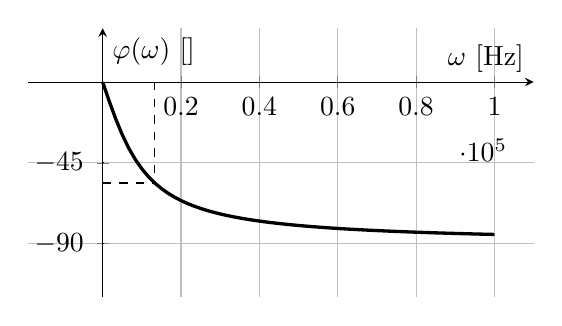
\begin{tikzpicture}
	\begin{axis}[
		xlabel={$\omega\ [\mathrm{Hz}]$},
		ylabel={$\varphi(\omega)\ [\degree]$},
		xmin=-19e3, xmax=1.1e5, % xmin < domain_min for yaxis description space
		domain=0:1e5, 
		ymin=-120, ymax=30,
		samples=61,
		axis x line=center,
		axis y line=center,
		width=8cm,
		height=5cm,
		%ytick={},
		yticklabels={}, % custom as nodes which are cut off (clip=true) otherwise width of axisbox changes and doesn't fit other plot
		ytick distance = 45,
		grid=major, % doesnt work ... maybe due to no y ticks
	]     
		\addplot[mark=none,very thick,]   {atan(-(x*1.25*1e-6*100*900)/(1000))}; % 1/(1+(omega*100*100*10^-6)^0.5)^2 % 100 Ohm, 100 uF
			%node [pos=0.45,anchor=south] {$\varphi(\omega)\ [\degree]$}; % plotlabel
		\addplot[black,thin] coordinates{(-20,-90)(20,-90)} node[anchor=east,black] {$-90\ $}; % yaxis tick
		\addplot[black,thin] coordinates{(-20,-45)(20,-45)} node[anchor=east,black] {$-45\ $}; % yaxis tick
		\addplot[dashed,thin] coordinates{(1.3304*1e4,0)(1.3304*1e4,-56.25)}; 	% berechnet in aufgabe c)
		\addplot[dashed,thin] coordinates{(0,-56.25)(1.3304*1e4,-56.25)}; 		% berechnet in aufgabe c)
	\end{axis}
\end{tikzpicture}%
